\chapter{Basic operations} \label{chap:basicop}


    \section{Introduction} 

This chapter introduces some of the most basic ingredients that support the programming.
Data types, data structures, maths operators or flow structures are some of the most basic concepts needed to code in any programming language. 
But first let's put them in context. 

An algorithm in mathematics is a finite sequence of unambiguous instructions to solve a specific problem. 
Notice that this definition involves that the algorithm ends in a finite number of steps, 
the sequence of instructions that yields the output are numbered and followed in their numerical order and
inputs, instructions and outputs must be properly identified. 

The problem can be seen as a function between a bunch of inputs and their associated outputs.
If we particularize it on a specific set of inputs we have an instance of that problem, 
then, we need an algorithm to solve the instance.
The theory of computation gives the basis for the automatic processing of the algorithm where there is a 
problem to solve, an algorithm that solves it and a machine to compute it. 

To take advantage of the use of machines that compute the algorithm automatically we use programs.
The program or code is the translation of the algorithm expressed in a mathematical language to a language understood by 
the machine, the programming language. 

Cuento los elementnos basicos de un programa que emulan el algoritmo
Cuento las caracteristicas fundamentales de un lenguaje de programacion


Notice that the \textit{variables} in a programming language imitate the \textit{memory cells} of the von Neumann architecture.
The \textit{control statements} emulate the \textit{jump and test instructions} and
the \textit{assignment statement} imitate the \textit{fetching, performing arithmetic and storing process}. 

The assignment statement \texttt{v = 3*5 + 2} becomes the bottleneck of programming languages in the sense that a program is mainly concerned 
with the flow of assignments of single variables (imitating single words). 
By executing assignments many times, maybe altering subscripts (imitating memory addresses), 
the program ends up with the result stored in a variable (imitating the storage in memory). 
Furthermore, this assignment statement splits the programming languages into two worlds: 
a world of expressions with strong algebraic properties (\texttt{3*5 + 2}) and a world of statements with few mathematical properties (\texttt{v =}).








    \section{Data types} 



Each constant, variable, array or function in a programming language has an intrinsic data type associated. 
This type decides, among other things, the permitted values that the entity can have and the set of operations that can be performed with them.
For example, the set of integers in mathematics are represented in a programming language through \texttt{integer} data type. 
Then, a value $x\in \mathbb{Z}$ will be stored in an \texttt{integer} variable and operations like addition, multiplication or exponentiation are allowed. 

The data typing in a programming language is explicit when the programmer needs to decide and declare the type for each variable or implicit when the language assumes the type. 
Furthermore, while some programming languages allow the use of some data types as if they were a different type (weak typing) others does not (strong typing). 
Python is mainly an implicit typing language since we can assign a value to a variable without declaring type, i.e. \texttt{a = 3} will automatically treat \texttt{a} as an integer. 
Fortran, on the contrary, is a explicit typing language because all variables must be previously declared with a specific type, i.e. \texttt{real :: x = 5.6}.




Notice that Fortran provides five intrinsic data types. 
Derived data types can be created either from intrinsic data types or from other derived types previously defined.
The five intrinsic types are:
\begin{itemize}
    \item Numeric nature: \texttt{integer}, \texttt{real}, \texttt{complex}. 
    \item Boolean nature: \texttt{logical}.
    \item Text nature: \texttt{character}.
\end{itemize}
The numeric types of data behave like the mathematical abstractions of these sets, 
roughly speaking: $n\in \mathbb{Z}$ is stored in an \texttt{integer}, $x\in \mathbb{R}$ is stored in an \texttt{real} and $z\in \mathbb{C}$ is stored in an \texttt{complex} variable.
The \texttt{logical} type gets the two possible values of the Boolean algebra; \texttt{True} and \texttt{False}. 
Finally, the \texttt{character} type can store strings with ASCII characters which includes alphanumeric, symbols and sign characters.   




The same data types are built-in in Python but with a different name (\texttt{int}, \texttt{float}, \texttt{complex}, \texttt{bool} and \texttt{str}). 
In addition, more data types can be found by default, among others we find:
\begin{itemize}
    \item Sequence nature: \texttt{list}, \texttt{tuple} or \texttt{range}.
    \item Mapping nature: \texttt{dict}.
    \item Set nature: \texttt{set}, \texttt{frozenset}.
\end{itemize}
These new types are used to store collections of data whose the elements can be any type of data. 
For example a list can contain strings together with integers or reals but also other lists nested. 
Notice that Fortran does not include these data types.




%MATEMATICAS:
%List/Sequence: enumerated collection of objects in which repetitions are allowed and order matters. USUALLY INFINITE
%Tuple: enumerated collection of objects in which repetitions are allowed and order matters. ALWAYS FINITE

%PROGRAMMING PYTHON:
%List/Sequence: enumerated collection of objects in which repetitions are allowed and order matters. ONLY FINITE IS POSSIBLE
%Tuple: Same as list but it can not change (programming concept not related to maths)

A \texttt{list} extracts its meaning from the concept of sequence/list in mathematics, notice that when talking about programming, lists can not be infinite while sequences can in mathematics:

\textit{A sequence is an enumerated collection of objects in which repetitions are allowed and order matters.}

Hence, a list is characterised by being i) ordered; the position within the list is kept, ii) changeable; change, add, and remove items are allowed when needed in the execution of the code and iii) allow duplicates; items can appear more than one time in the list. Notice that the difference between any two elements comes with the index within the list.
A \texttt{tuple} is quite the same than a \texttt{list}: ordered data collection that allows duplicates. 
%takes also the mathematical meaning: \textit{a finite ordered list (sequence) of elements} 
However, tuples are unchangeable, which means that once created we cannot change, add or remove items. 
Python allocates the required memory once and not reallocates it so this becomes a more memory efficient strategy to follow when the data is going to be immutable.

A list is written using square brackets and a tuple round brackets, both with comma-separated values:
\begin{verbatim}
L = [ ("one", 5, 3.5, 5 ]
\end{verbatim}
\begin{verbatim}
T = ( ("one", 5, 3.5, 5 )
\end{verbatim}

A \texttt{set} in Python takes the same meaning as the definition of set in the set theory started by Georg Cantor:

\textit{A set is a gathering together into a whole of definite, distinct objects of our perception or our thought, which are called elements of the set.}

Hence, Python treats them as a collection of any type of data, but in this case i) unordered and ii) not allowing duplicate values. 
In a set, all that matters is whether each element is in it or not, so the ordering of the elements is irrelevant (there is not an integer index pointing to them).
Furthermore, notice that two equal elements, since they are not ordered, could not be distinguished between them. Hence, duplicate values are not allowed. 

Roster or enumeration notation defines a set by listing its elements between curly brackets separated by commas:
\begin{verbatim}
S = { 4, 2, 1, 3 }
\end{verbatim}
\begin{verbatim}
S2 = { blue, white, red }
\end{verbatim}
As it is easy to follow from the definition, different orderings in roster notation does not change the set.
For example, $\{ 2, 4, 6 \}$ and $\{ 4, 6, 4, 2 \}$ represent the same set.
For sets with many elements, especially those following an implicit pattern,
the list of members can be abbreviated using an ellipsis ``...''.
For instance, the set of the first thousand positive integers 
may be specified in roster notation as
\begin{verbatim}
{ 1, 2, 3, ..., 1000 }.
\end{verbatim}
In a set the data can be modified through built-in methods so for example mathematical set operations like union, intersection or difference can be performed.
Exactly like a tuple is an unchangeable list, a \texttt{frozenset} is an unchangeable set, once created, its content can not be modified. 

A dictionary (\texttt{dict}), like a list, is also a collection of data that can store any type of data (even other dictionaries nested), are ordered and changeable.
However, unlike lists, the values are stored in pars: \texttt{key:value} and do not allow duplicates; it cannot have two items with the same key.

To write a dictionary we write the list of elements, separated by commas and using a colon (\texttt{:}) to separate each pair. 
Also, all the content is enclosed in curly brackets (\texttt{\{\}}). 
Let's see an example:
\begin{verbatim}
D = { ``Name'': ``John'', ``Age'': 32, ``Mark'': 7.3 }
\end{verbatim}

\newpage
When we want to use all these collections of data, since they are treated as \textit{iterable} objects, we can use a \texttt{for} loop to iterate through them. 
If \texttt{V} is a list, tuple, dictionary or set, we can move throughout all the elements using:
\begin{verbatim}
for v in V:
\end{verbatim}
So \texttt{v} takes, sequentially, all the values stored in \texttt{V}. 
Notice that, if \texttt{V} is a set, the elements won't follow any specific order. 
Let's execute for example:
\begin{verbatim}
S = {7,2,"car",78.2,"boat",4.5}
for x in S:
    print(x)
\end{verbatim}
resulting in:
\begin{verbatim}
2
4.5
7
boat
78.2
car
\end{verbatim}
Use the following expression to iterate using an index throughout the whole length of the collection:
\begin{verbatim}
for i in range(len(V)): 
\end{verbatim}
or extract both the index and the value of the element using:
\begin{verbatim}
for i, v in enumerate(V):
\end{verbatim}




In the following examples the intrinsic data types in Fortran and Python are presented through some basic expressions. 


\newpage 
\subsection*{Fortran code}
Since Fortran is a explicit typing language, before using any variable, all must be previously declared with a specific type.
The following program shows an example of the declaration and initialization of the five data types we can find. 
%\vspace{0.5cm}
%\lstfor
%\renewcommand{\home}{./Fortran/sources/Advanced_programming/scope} 
%\listings{\home/modB.f90}{module modB}{end module}{modB.f90}

\begin{verbatim}
program data_types
    
    implicit none
    
    character (len=10,kind=1) :: string = 'data types'
    integer :: int = 1
    real :: x = 1.8
    complex :: com = (1,1)
    logical :: bool = .true.
    
end program
\end{verbatim}




\newpage 
\subsection*{Python code}
Take a look now at the example of use of these data types in Python. 
Essentially both codes are quite similar, 
however, now data types for variables are not explicitly declared because 
Python automatically declares them. 
In addition, indentation rules must be strictly followed. 
\vspace{0.5cm} 
\lstpython
\renewcommand{\home}{./Python/sources/Foundations/data_type} 
\listingsp{\home/data_type.py}{def}{format}{data_type.py}




 
    \section{Data structures} 
 
The following concepts regarding arrays constructions and operations are covered:
\begin{enumerate} 
    \item Type, rank and dimension of arrays.
    \item Constructors to initialize an array. 
    \item Sectors or slices of arrays. 
    \item Operations among array. 
\end{enumerate} 


Some basic notions are summarized now: 
%\begin{itemize}
%    \item An array is properly declared when it has type, rank and dimension (or extent). 
%All this information comes from the mathematical definition of the vectors and matrices.
%
%\begin{enumerate}
%    \item The data type in this case is \texttt{real} since the examples are built with real vectors/matrices. 
%    \item Rank is the number of dimensions in the array; a rank-one array represents a column vector (\texttt{V} or \texttt{W}), a rank-two array represents a matrix organised into columns and rows (\texttt{A} or \texttt{B}), etc. 
%    \item The extent of each particular dimension is its length, which means, the number of elements in that dimension. All dimensions involved in these examples are equal to \texttt{N}. The bounds of a dimension does not have to start with index \texttt{1}, later some examples with different bounds are shown. 
%\end{enumerate}
%
%\item Once declared, the initialization of the arrays is performed with constructors. In the case of Fortran the constructors are only used for rank-one arrays so functions like \texttt{reshape} are needed for higher ranks. Three ways are normally used to manually construct an array:
%
%\begin{enumerate}
%    \item By a list of values: \texttt{ [ list ] } where 'list' is full of values separated by commas (of the same type declared for the array). 
%    For example: 
%    
%    \texttt{V = [ 3.4, 5.2, 4.5, 2.1 ]} is a column vector of dimension 4 with those values in each position.
%    \item An array expression can also be used in the initialization: 
%    
%    \texttt{V = [ B(2, 3:5) ]} stores in \texttt{V} the list of values in the second row of \texttt{B} from columns \texttt{3} to \texttt{5}.
%    \item Using an implicit loop so a list of elements is computed from a loop controlled by a DO variable. Lots of examples of this are used throughout this book: \texttt{V = [ ( 1./i**2, i=1, N ) ]}.
%\end{enumerate}
%
%\item The sectors of an array are already introduced in this text. Notice that the initialization of \texttt{V} in this example: \texttt{V = [ B(2, 3:5) ]} use a sector of the whole array \texttt{B}. This can also be extended to a whole dimension of an array, i.e. the column 5 of an array \texttt{C} is referred like \texttt{C(:,5)}. Furthermore, alternate values can be selected by specifying a lower and upper bound and the jump between values (see matrix B of Figure \ref{fig:arrays}): \texttt{B(-2:4:2,:)} being the second value \texttt{2} the jump between rows.
%
%\begin{figure}
%    \begin{subfigure}[h]{0.5\textwidth}
%        
%        \centering
%        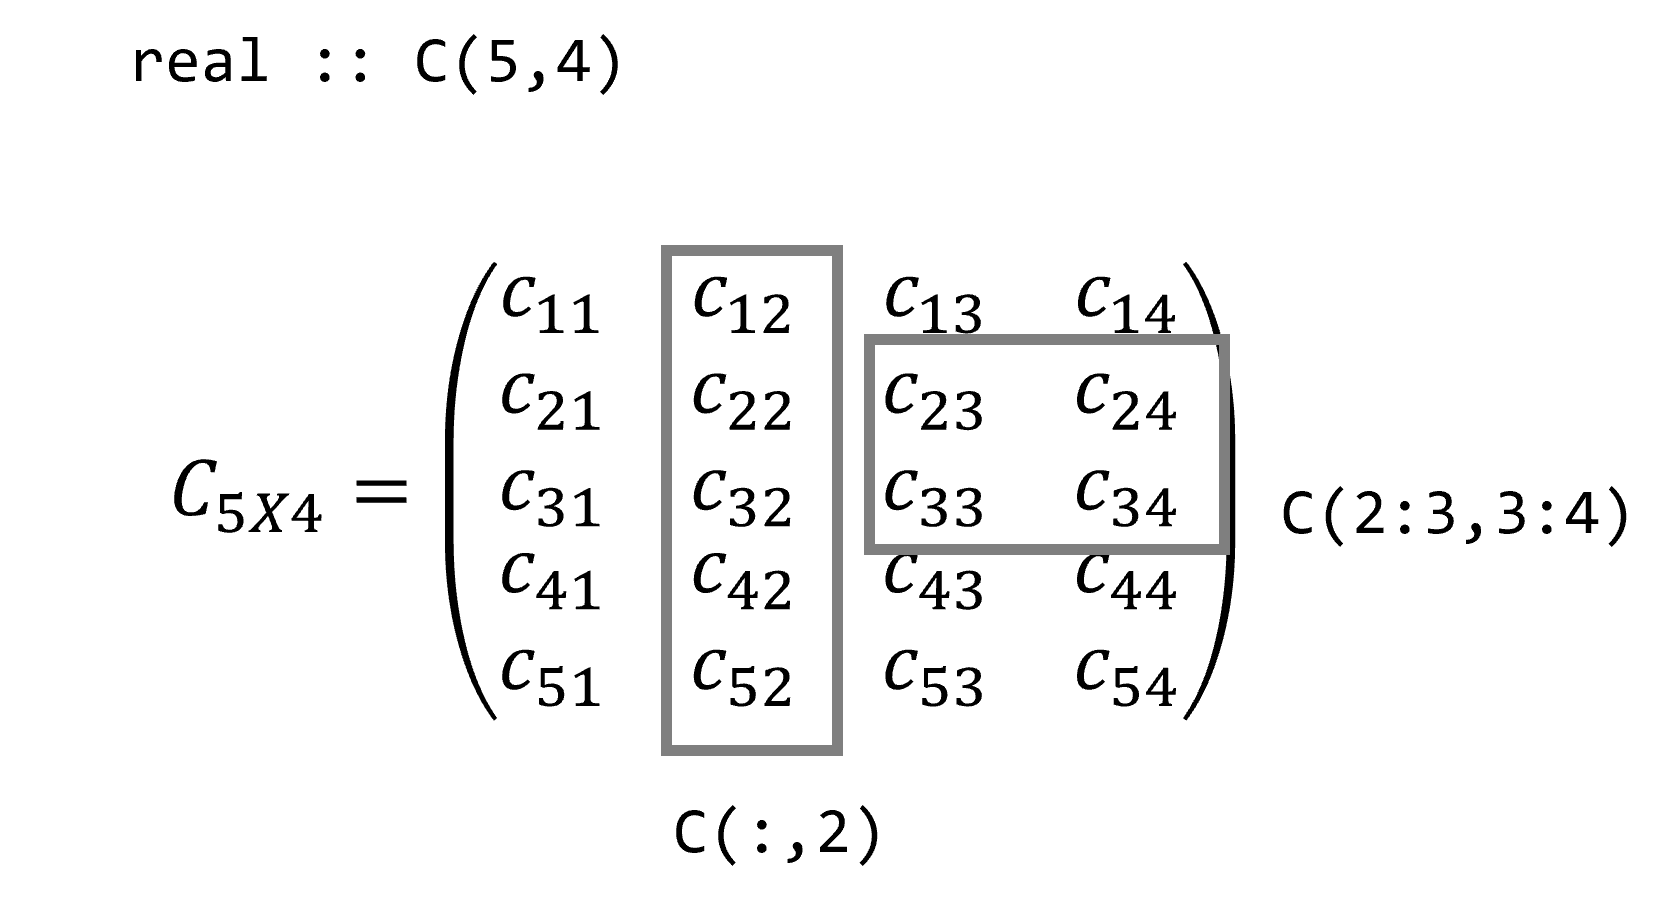
\includegraphics[width = \textwidth]{./doc/Figures/Array1.png}  \\
%        \begin{flushleft}
%            Rank = 2 \\
%            %Extent = 5 and 4 \\
%            Size = 20 \\
%            Bounds = (1:5, 1:4) \\
%            Shape = (5, 4)
%        \end{flushleft}
%        
%    \end{subfigure}
%    \hspace{\fill}
%    \begin{subfigure}[h]{0.5\textwidth}
%        
%        \centering
%        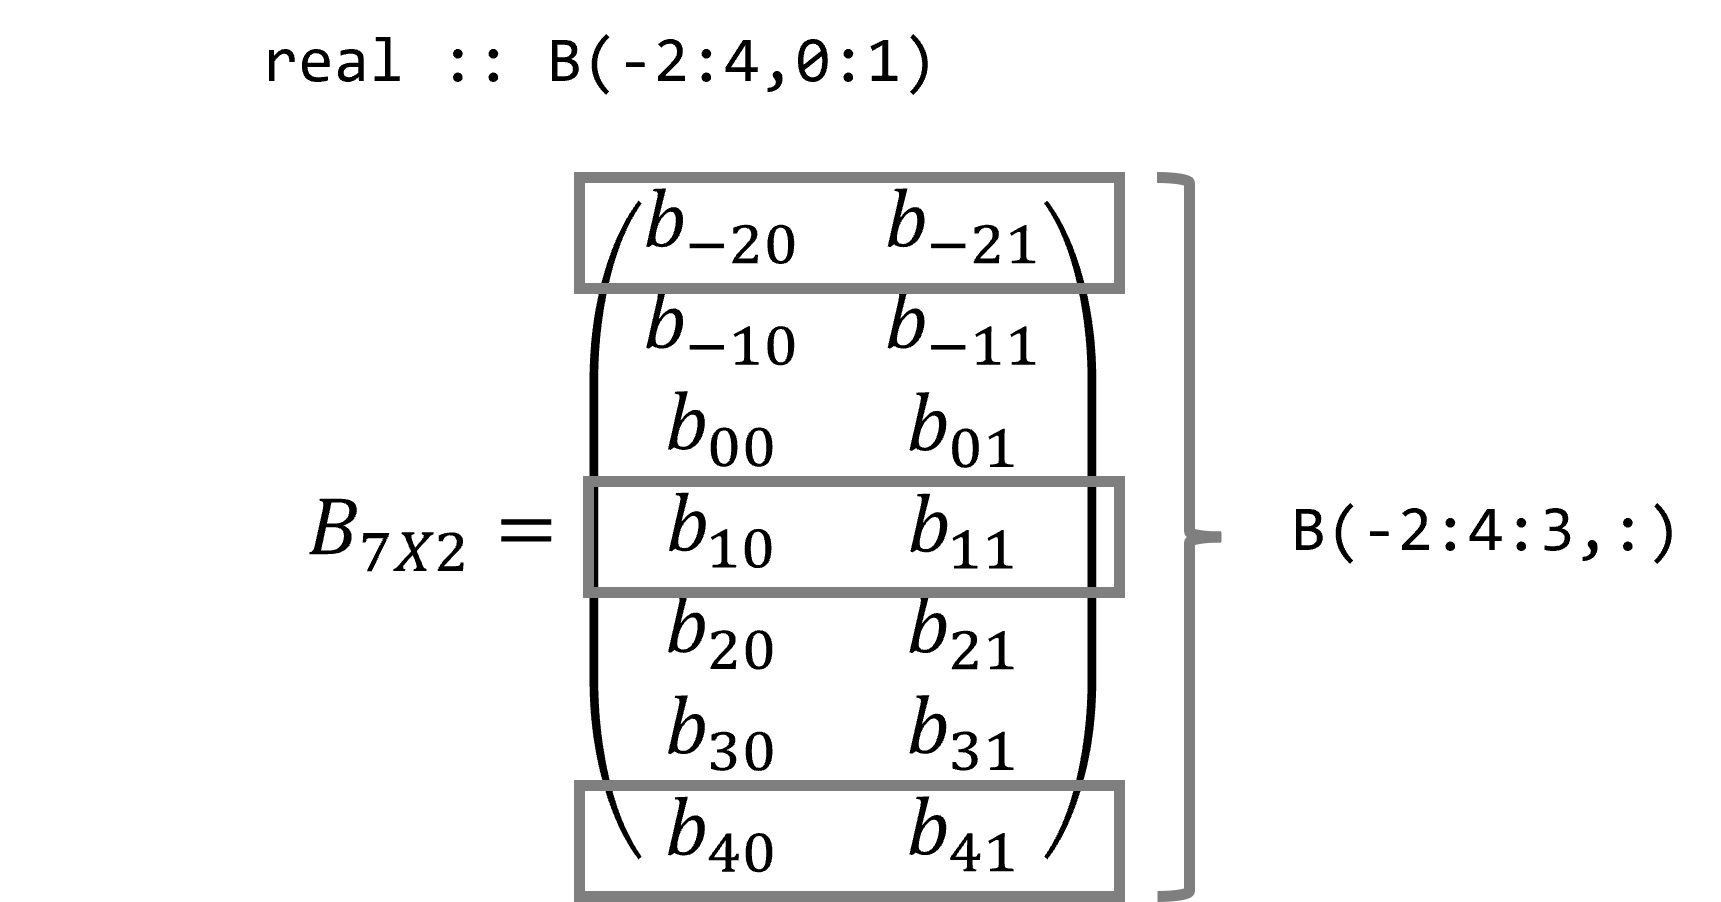
\includegraphics[width = \textwidth]{./doc/Figures/Array3.png}  \\
%        \begin{flushleft}
%            Rank = 2 \\
%            %Extent = 7 and 2 \\
%            Size = 14 \\
%            Bounds = (-2:4, 0:1) \\
%            Shape = (7, 2)
%        \end{flushleft}
%        
%    \end{subfigure}
%    \caption{Properties of a couple of arrays.}   \label{fig:arrays}
%\end{figure}
%
%\end{itemize}


%\texttt{ (/ list /) } is not used as constructor.





\newpage
    \section{Maths operators}
Arithmetic operator 
Comparison operator 
Logical operator 
Membership operator 

    \section{Assignment operators}


    \section{Flow structures}

if 
where 
iterators: list, tuples, arrays, sets, dictionaries (key, value)



for k in D   dictionary iterates in key 
for k in D.keys()   dictionary iterates in keys
for v in D.values()   dictionary iterates in values


\newpage 
    \section{Roots of a second degree equation} 
In this section, a program to obtain the roots of a second order equation is presented:  
$$
a x^2 + b x + c = 0, \qquad \forall \ a, b, c \in \mathbb{R}.
$$
The fundamental theorem of algebra states that every  Nth order polynomial has N complex roots. 
If the coefficients are real, then the roots are complex conjugate.
Dividing the above equation by $ a $ an looking for a perfect square, 
the following equation is obtained: 
$$
\left( x + \frac{b}{2a} \right)^2 - \frac{b^2 }{ 4 a^2} + \frac{c}{a} = 0. 
$$
Solving the unknown $x$, the well known formula for the roots is obtained: 
\begin{equation}
 x_{1,2} = \frac{ - b \pm \sqrt{ b^2 - 4 a c }  }{ 2 a  }  
 \label{x12}
\end{equation} 
If the discriminant $ d = b^2 - 4 a c $ is less than zero, roots become complex. 
In the following code, complex solutions given by (\ref{x12}) are implemented. 
Note that the discriminant $ d $ was defined as a complex variable to avoid math problems 
when the discriminant is negative. Whereas the root of a real negative number is not defined,
the root of a negative number has a value for complex numbers. 
 
\vspace{0.5cm}
\renewcommand{\home}{./Fortran/sources/Foundations/Roots} 
\lstfor
\listings{\home/Roots.f90}{subroutine Roots_2th}{end subroutine}{Roots.f90}


\newpage 
\subsection*{Python code}
The same function is presented below coded with Python. Essentially both codes are quite similar, 
however, now data types for variables are not explicitly declared because 
Python automatically declares them. In addition, indentation rules must be strictly followed. 
\vspace{0.5cm} 
\lstpython
\renewcommand{\home}{./Python/sources/Foundations/Roots} 
\listingsp{\home/Roots.py}{from}{output}{Roots.py}
%\lstfor
  
  
 
 
